% DOCUMENT PREAMBLE
\documentclass{emulateapj}
% \documentclass[referee]{apj}

\usepackage{graphicx}
\usepackage{float}

\usepackage{subcaption}

\usepackage{apjfonts}
\usepackage{microtype}

\begin{document}

\title{Solar jet observed at the limb in SDO/SST}
\author{S.M.Bennett$^1$
and
\author A.J.Leonard$^1$}
\affil{$^1$ Solar Physics and Space Plasma Research Centre (SP2RC), University of Sheffield, Hicks Building, Hounsfield Rd, S3 7RH, UK}


\begin{abstract}
\end{abstract}

\maketitle

\section{Introduction}
Solar jets of various forms are ubiquitous the solar atmosphere, from spicules low in the chromosphere to macropsicules passing through the transition region and X-Ray jets extending into the solar corona. 
Investigations into these phenomena have advanced significantly with recent developments in solar telescopes such as Hinode and the Solar Dynamic Observatory.
These features are observed in a range of wavelengths and heights in the atmosphere. 

Low in the chromosphere a predominant feature is the spicule, these small scale jets, generally forming at the inter-granular lanes and reaching heights of $1$ - $5$ Mm.
They are also very short lived with a maximum lifetime of ~$5$ mins.
More importantly there is currently debate as to whether the population of spicules is divided into two forms, Type-1 and Type-2. 
Type-1 are described as longer lived and less explosive with respect to velocity, whereas Type-2 reach higher velocities and higher into the atmosphere, however are not observed to fall back down \cite{DePontieu2007}. 

Having stated this, \cite{Pereira2014} have revealed that Type-2 spicules disappearance may be as a result of heating and moving out of the passband, due to the fact that they are consequently observed in a hotter line which may imply that these features are not in fact separate populations and \cite{Zhang2012} finds no such distinction in population.

Many formation mechanisms have been proposed for spicules, including reconnection, p-mode driving and applying accretion disk models in a solar context, for a review see \cite{Sterling2000}.
More recently the question surrounding spicules is how they contribute to the atmosphere, this is particularly pertinent given their vast number, any contribution they make would be scaled up by their sheer ubiquity.
\cite{Rouppe2015} used coordinated observations with SST and IRIS to study RRB's and RBE's, examining H$\alpha$, Mg II h \& k, C II and Si IV.
The authors find that these spicule-like extensions observed in H$\alpha$ have counter parts in the hotter Magnesium lines and the upper chromosphere/transition region C II and Si IV, which would certainly imply that these features are heating either themselves or the atmosphere around them.

These spicules are similar to other features such as surges, the already mentioned RRB's/RBE's and chromospheric jets, all of which need considering in terms spicules \citep{Tsiropoula2012}.


Higher in the chromosphere, we find macrospicules. 
Larger counterparts of spicules, initially observed in $1975$ by \cite{Bohlin1975} using the Skylab 2 mission using a He $30.4$ nm filter viewing the upper chromopshere.
Bohlin stated their lifetimes to be $5$ to $30$ mins and lengths to be approximately $10$ - $50$ arcsec, and these values have been backed up by more modern studies such as \cite{Bennett2015}.

Macrospicules are generally accepted as multi thermal structures, featuring a cool core and a hot sheath, from being observed in H$\alpha$ \citep{LaBonte79} and hotter high chromosphere lines such as in \cite{Parenti2002}.
They have also been observed to rotate, \cite{Pike_Mason1998} and \cite{Kamio2010}, the latter paper quotes $-120 \pm 15$kms$^{-1}$ blue shift doppler velocity on the left side of the macrospicule. 

There are multiple proposals for the mechanism triggering apparent rotation of the macrospicule, \cite{Curdt2011} propose that the Suns differential rotation causes macrospicules rotation, whereas, reconnection events causing the relaxation of a small scale twisted loop is demonstrated by \cite{Adams2014}.
Again, with macrospicules extending high into the atmosphere, the question of their effect upon it, is one that needs answering.
\cite{Pike_Harrison1997} observe outflows from the macrospicule of the order $2002$ kms$^{-1}$ in He I and discuss whether these outflows could potentially accelerate the solar wind.
However, work by \cite{Zaqarashvili2014} question whether jets moving at super-alfvenic speeds might cause a Kelvin-Helmholtz stability to form at the macrospicule/atmosphere boundary, which would, in turn, transport heat into the corona.

A third  category are coronal jets, observed in slightly hotter lines but still EUV such as those discussed in \cite{Shibata1992}.
Here they are described later in \cite{Shibata1994} as reconnection events, where reconnection is triggered by flux emergence at the base of a small scale loop.
However after this reconnection, there are several models as to how the system will evolve.
\cite{Moore2010} demonstrate a dichotomy in formation mechanism of coronal jets, between the standard 'inverted Y' model demonstrated by Shibata and the blowout jet model. 
This model differs from the standard model, in this case the reconnection leads to a 'curtain' of plasma flow as opposed to the 'spire' from the standard model.
The difference between the two models originates in initial configuration of the overlying arch. 
In standard jets the arch has no appreciable shear, whereas for a blowout jet the arch is twisted and sheared sufficiently to drive the explosive outflow which forms the jet.
Coronal jets have also been shown to accelerate particles into interplanetary space \citep{Li2011}, there is also evidence for repeat onset jets, with several re-occurrences, see \cite{Li2011} and \cite{Chifor2008} demonstrate repeat on-set of jets driven by flux cancellation.

Lastly we need to consider X-ray jets.
\cite{Shimojo2000} define their physical properties studying 16 separate jet events.
Due to limitations on instrumentation at the time, the authors do not cover the extent of the jets, however, their analysis covers temperature, $3 - 8$ MK, and density, $0.4 - 4.0$ cm$^{-9}$.
The authors also discuss flaring at the foot-point of X-ray jets, in that, the temperature is proportional to the size of the initial footpoints.

\cite{Kamio2010} applied a great deal of the background above when studying a macrospicule and X-ray jet simultaneously forming. There is also discussion in \cite{Pike_Harrison1997} and \cite{Kim2007} on the appearance of X-ray jets, alongside small scale jets.

In the following sections we aim to comprehensively discuss the physical properties of our case study. In \ref{obs_sect} we will present the observations we are using. \ref{time_dist_sect} will discuss the evolution of the jet with respect to its extent. We will then move on to a doppler analysis of the jet in \ref{dop_shift_sect}. Lastly we will attempt to quantify the effect of the jet on the atmosphere in \ref{temp_map_sect} before making our conclusions.

 
 




% % % % %Things to talk about in the introduction
% xray jets
% Formation models for all of the things



\section{Observation}
\label{obs_sect}
We observed a jet-like (hereby referred to as 'the jet') feature at the limb on $21st$ June 2016 beginning at $07:30:00$ in the Crisp Imaging Spetrapolarimeter (CRISP), an instrument installed on the Swedish Solar Telescope (SST) during a period of good seeing. %cite scharmer et al 2003
We used the H$\alpha$ filter, core line $656.28$ nm with $35$ slit increments from the core covering a $.32$ nm range, $-0.2$ and $+0.12$, and were further processed using te Multi-Object Multi-Frame Blind Deconvolution (MOMBFD \cite{vanNoort2005}).
The observations were of active region AR 11506 with $xc = 893, yc = -250$ in heliocentric coordinates on $930x930$ pixel images, with spatial resolution on $0.012$ arcsec/pixel and temporal resolution on $7.5$ sec.
Due to the constant surveillance we currently have the Sun under, we also have simultaneous observations with the Solar Dynamic Observatory (SDO) and the Solar Terrestrial Relations Observatory (STEREO).

Using the Atmospheric Imaging Assembly (AIA), we observe the jet in most of the wavelengths available, $30.4$, $35.5$, $211$, $17.1$ and $13.1$ nm.
AIA on-board SDO \cite{AIAspec} provides $4096 \times 4096$ pixel images with a spatial resolution of $0.6$ arcsec per pixel and a cadence of $12$ sec.

Lastly, we also have observations in STEREO using the Heliospheric Imager \citep{Defise2001}. 
We are fortunate that when these observations were taken, STEREO A was at approximately $90^\circ$ to the Sun-Earth line, as such we also have observations of this feature as an on-disk feature.
In this case we are using the $30.4$ nm HI instrument, however, the distance from the Earth has now reached a point that the temporal cadence has reduced to $10$ min.
While this is possibly too high to undertake a detailed examination, we can certainly utilise this method to inform us as to the global behaviour of the macrospicule.
As we have a suite of observing instruments to utilise we aim to build a comprehensive description of this feature and how it may affect the environment around it.


\section{Time Distance Evolution}
\label{time_dist_sect}


Let us begin with the evolution of the jet feature over time. 
We have utilised a self-built, manual feature measuring tool, which, uses a clicking mechanism to select the foot and tip of the macrospicule, calculates the half weight and uses this as a guide to measure the width of the feature.
Using this tool on each frame, and therefore the time cadence of the instrument, we obtain the evolution of the jet and general ballistic information.
We have used this tool on each wavelength to examine the extent upwards through the corona. 

\subsection{Onset}
The jet feature is observed in high resolution as it forms using SST and, fortunately, we can resolve initial stages of the jet formation.
The jet is observed to initiate in the core of H$\alpha$ with two small bright points forming, and an ensuing jet developing above it. 
This behaviour is in keeping with the standard jet formation model demonstrated by \cite{Shibata1992}, where the authors describe an 'inverted y' shape of brightened material that is a result of small scale flux emergence reconnection.

Observations in SDO record the entire lifetime of the feature, however the same is not true for observations using the SST, where the observation window in SST closes at $07:48:00$.



\subsection{STEREO-A}
We are fortunate that we can observe the jet feature in the STEREO-A Heliospheric Imager (HI), with the position of the spacecraft at approximately $90\deg$ to the Sun-Earth line.
This facilitates the building of a larger picture of the behaviour of the jet, the downside to this however, is that with STEREO-A being at such a distance the cadence is low, $~10$ mins.
In this case we obtain 4 images in $30.4$ nm in which the jet is observed

\begin{figure}[]
	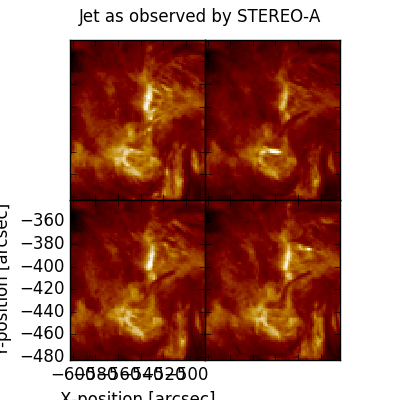
\includegraphics[width=\columnwidth]{../figures/STEREO-A.png} 
	\caption{HI $30.4$ nm images at $07:26:15$, $07:36:15$, $07:46:15$ and $07:56:15$ going from left to right.}
\end{figure}




\section{Doppler shift}
\label{dop_shift_sect}




\section{Temperature Maps}
\label{temp_map_sect}







\section{Discussion \& Conclusion}



\bibliographystyle{apj}
\bibliography{references}







\end{document}